\documentclass[11pt]{article}
\usepackage[dvipsnames]{xcolor}
\usepackage{times}
\usepackage{amsmath,amsthm,amssymb,setspace,enumitem,epsfig,titlesec,verbatim,array,eurosym,multirow}
\usepackage[sort&compress,numbers]{natbib}
\usepackage[footnotesize,bf]{caption}
\usepackage[margin=2.5cm, includefoot, footskip=30pt]{geometry}
\usepackage{standalone}
\usepackage{tikz}
\usepackage{subcaption}
\usepackage{hyperref}
\usepackage{tabularx}
\usepackage{booktabs}
\usepackage{blkarray}
\usepackage[ruled,vlined]{algorithm2e}
\smallskip % Erlaubt kleine Abstaende zwischen Paragraphen, falls es dem Seitenlayout hilft
\renewcommand{\baselinestretch}{1.15}
\usepackage{tikz}
\usetikzlibrary{arrows}
\usepackage{minitoc}
\usepackage{graphicx}
\usepackage{hyperref}
\usepackage{subcaption}
\usepackage{multirow}
\usepackage{multicol}
\usepackage{standalone}

\newcommand{\nikoleta}[1]{\textcolor{orange}{\textbf{NG}: #1}}
\newcommand{\christian}[1]{\textcolor{blue}{\textbf{CH}: #1}}

\newtheoremstyle{plainCl1}% name
{12pt}%      Space above, empty = 'usual value'
{12pt}%      Space below
{\it}% 	   Body font
{}%         Indent amount (empty = no indent, \parindent = para indent)
{\bfseries}% Thm head font
{}%        Punctuation after thm head
{\newline}% Space after thm head: \newline = linebreak
{}%         Thm head spec

\theoremstyle{plainCl1}
\newtheorem{theorem}{Theorem}
\newtheorem{lemma}{Lemma}
\newtheorem{corollary}{Corollary}
\newtheorem{proposition}{Proposition}


\newtheoremstyle{plainCl2}% name
{12pt}%      Space above, empty = 'usual value'
{12pt}%      Space below
{}% 	   Body font
{}%         Indent amount (empty = no indent, \parindent = para indent)
{\bfseries}% Thm head font
{}%        Punctuation after thm head
{\newline}% Space after thm head: \newline = linebreak
{}%         Thm head spec

\theoremstyle{plainCl2}
\newtheorem*{definition}{Definition}



\def\wsls{\texttt{WSLS}}
\def\tft{\texttt{TFT}}
\def\gtft{\texttt{GTFT}}
\def\allc{\texttt{ALLC}}
\def\alld{\texttt{ALLD}}
\def\alt{\texttt{Alternator}}



\titleformat{\section}{\sffamily \fontsize{12}{15}\bfseries}{\thesection}{0.4em}{}
\titleformat{\subsection}{\sffamily\fontsize{11}{15}\bfseries}{\thesubsection}{0.4em}{}
\renewcommand{\thefigure}{S\arabic{figure}}


\title{~\\[-1.5cm]{\sffamily \Large Revision notes}\\[-0.3cm]}

\date{\empty}

\begin{document}
%% DEFECTING STRATEGIES: Donation Game %%

\section{Reactive defecting Nash strategies in the donation game}\label{section:defecting_donation_game}

In the previous section, we have characterized the reactive partner strategies
for a special case of the donation game and the general prisoner's dilemma. In
the following, we apply the same methods to
characterize defecting Nash equilibria. For the case of reactive-1 strategies, we
obtain the following characterization.

%% DEFECTING STRATEGIES: Reactive-1 Donation Game %%

\begin{theorem}[Reactive-1 defecting Nash strategies in the donation game]
\label{theorem:reactive_one_defecting_strategies}
A reactive-1 strategy $\mathbf{p}$ is a defecting Nash strategy if and only if
its entries satisfy the conditions

\begin{equation}
  \begin{array}{rcl}
    p_{C} \le  \frac{c}{b} \qquad \text{ and } \qquad  p_{D} \!=\! 0.
\end{array}
\end{equation}
\end{theorem}


%% DEFECTING STRATEGIES: Reactive-2 Donation Game %%

\begin{theorem}[Reactive-2 defecting Nash strategies in the donation game]
\label{theorem:reactive_two_defecting_strategies}
A reactive-2 strategy $\mathbf{p}$ is a defecting Nash strategy if and only if
its entries satisfy the conditions

\begin{equation}\label{eq:defecting_conditions_two}
  p_{CC} \le \frac{c}{b}, \qquad \displaystyle \frac{p_{CD} \!+\! p_{DC}}{2} \le \frac{c}{2b}, \qquad p_{DD} = 0.
\end{equation}
\end{theorem}

%% DEFECTING STRATEGIES: Reactive-3 Donation Game %%

\begin{theorem}[Reactive-3 defecting Nash strategies in the donation game]
\label{theorem:reactive_three_defecting_strategies}
A reactive-3 strategy $\mathbf{p}$ is a defecting Nash strategy if and only if
its entries satisfy the conditions

\begin{align}\label{eq:defecting_conditions_three}
  \begin{split}
  p_{CCC} & \le \frac{c}{b} \\
  \frac{p_{CDC} + p_{DCD}}{2} & \leq \frac{1}{2} \cdot \frac{c}{b} \\
  \frac{p_{CCD} + p_{CDC} + p_{DCC}}{3} & \leq \frac{2}{3} \cdot \frac{c}{b} \\
  \frac{p_{CDD} + p_{DCD} + p_{DDC}}{3} & \leq \frac{1}{3} \cdot \frac{c}{b} \\
  \frac{p_{CCD} + p_{CDD} + p_{DCC} + p_{DDC}}{4}  & \leq \frac{1}{2} \cdot \frac{c}{b}  \\
  p_{DDD} & = 0.
  \end{split}
\end{align}

\end{theorem}

We repeat the same analysis for reactive counting strategies. We obtain the
following results.

%% DEFECTING STRATEGIES: Reactive-2 Counting Donation Game %%

\begin{theorem}[Reactive-2 defecting Nash counting strategies in the donation game]
\label{theorem:reactive_two_defecting_counting_strategies}
A reactive-2 counting strategy $\mathbf{r}$ is a defecting Nash strategy if and only if
its entries satisfy the conditions

\begin{equation}\label{eq:defecting_conditions_two_counting}
  r_{2} \le \frac{c}{b}, \qquad \displaystyle r_{1} \le \frac{1}{2} \cdot \frac{c}{b}, \qquad r_{0} = 0.
\end{equation}
\end{theorem}

%% DEFECTING STRATEGIES: Reactive-3 Counting Donation Game %%

\begin{theorem}[Reactive-3 defecting Nash counting strategies in the donation game]
\label{theorem:reactive_three_defecting_counting_strategies}
A reactive-3 counting strategy $\mathbf{r}$ is a defecting Nash strategy if and only if
its entries satisfy the conditions

\begin{equation}\label{eq:defecting_conditions_three_counting}
  r_{3} \le \frac{c}{b}, \qquad r_{2} \leq\frac{2}{3} \cdot \frac{c}{b}, \qquad
  r_{1} \leq\frac{1}{3} \cdot \frac{c}{b}, \qquad
  r_{0} = 0.
\end{equation}

ToDo: proofs.
\end{theorem}


\noindent
We can observe that for each value of \(n\), the left-hand side of the
conditions for cooperative and defective Nash are the same. Moreover, we see
that the right-hand side of the defective Nash conditions is always
strictly smaller than those of the cooperative Nash conditions. This means that
within the space of feasible strategies, the volume of partner strategies is
always larger than the volume of defective Nash strategies. We also verify this
analytical results numerically, Figure~\ref{fig:reactive_volume}.

\begin{figure}[t]
  \centering
  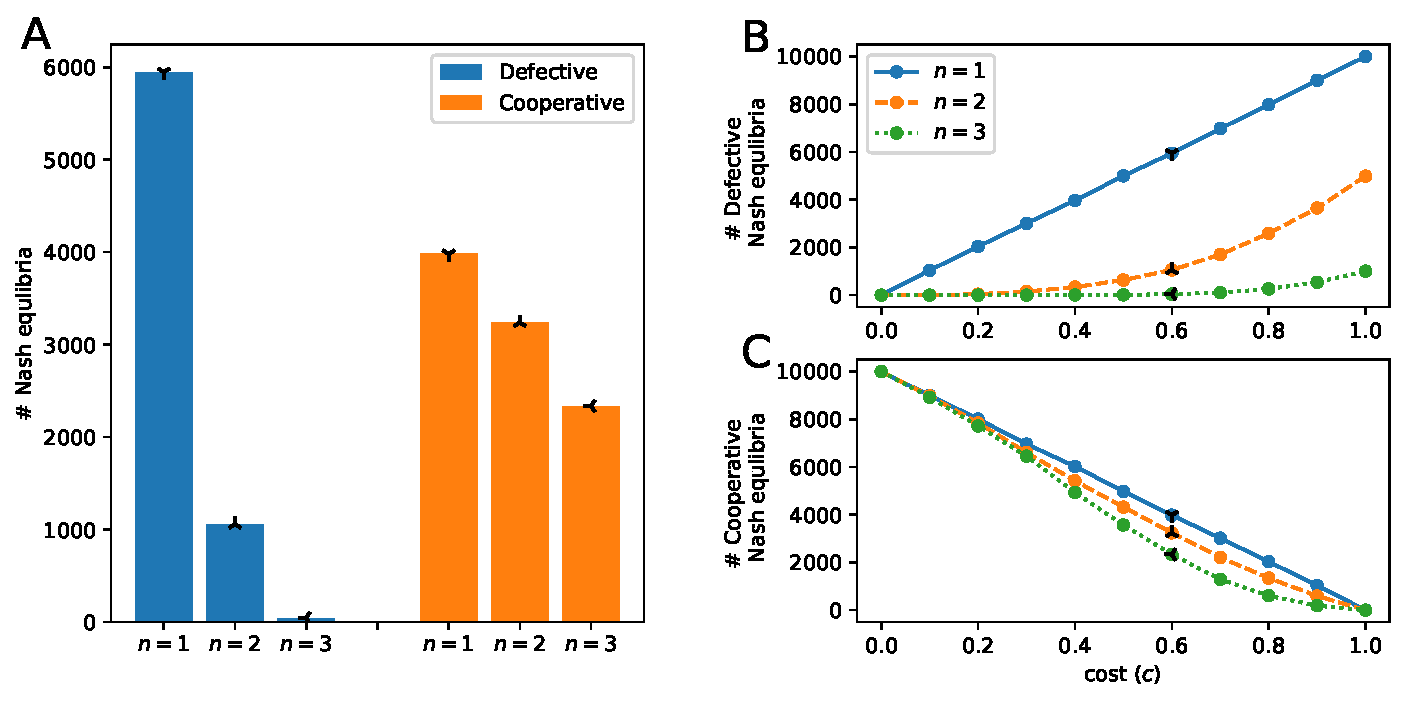
\includegraphics[width=\textwidth]{../../figures/siFig1.pdf}
  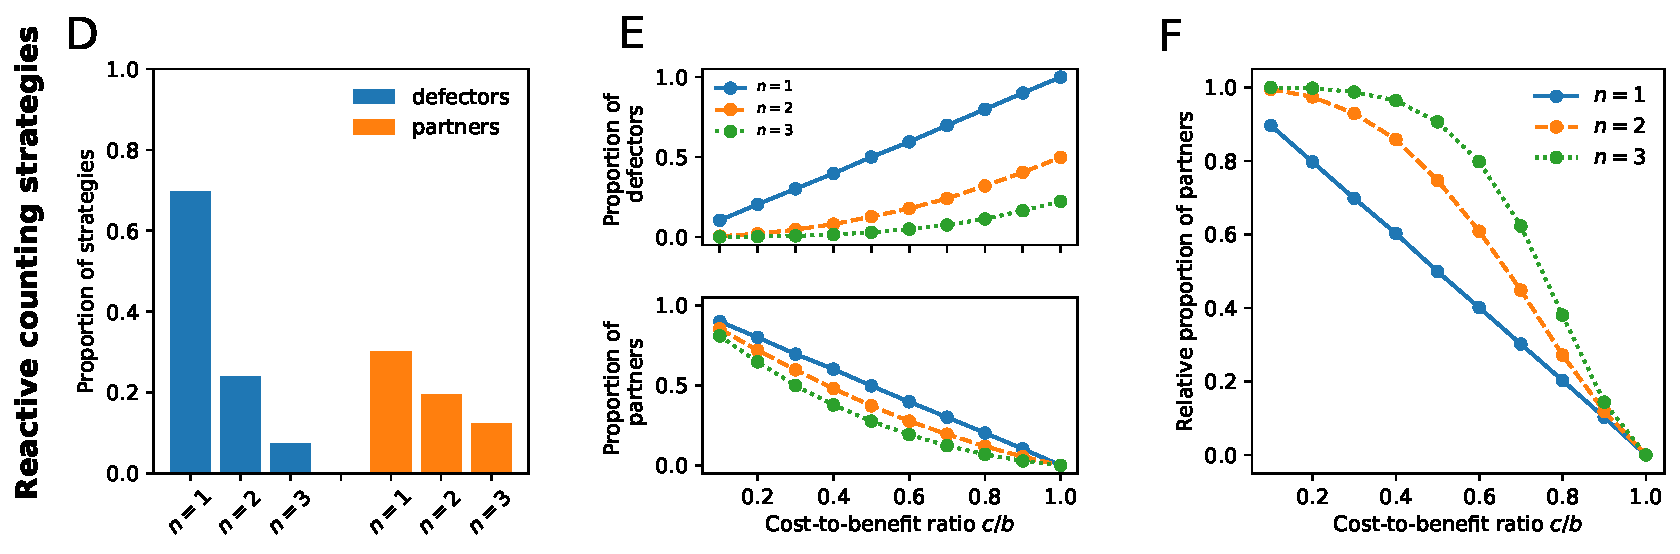
\includegraphics[width=\textwidth]{../../figures/siFig1Counting.pdf}
  \caption{
  \textbf{Volume of cooperative and defective Nash.}
We draw \(10^4\) random
strategies from the feasible space of strategies and create two copies of each
strategy. For one copy, we set the probability of cooperating after full
cooperations of the co-player to 1. For the second copy, we set the probability
of cooperating after full defections of the co-player to 0. We then checked if
either copy is Nash: cooperative for the first copy and defective for the second.
We set the benefit of cooperation to \(b = 1\).
{\bf A, D} We plot the results for a given value of cost, \(c = 0.5\). We do this
for reactive strategies and reactive counting strategies. For $n=1$, we can see
the number of defective equilibria is higher than that of the cooperative.
Howver, as we increase $n$ this is not true anymore. The number of defective
Nash decreases drastically. The number of partner strategies does as well,
howber, we can see that it happends less quickly.
{\bf B} We plot the porpotion of equalibria
over different values of cost, for reactive (B) and reactive counting strategies.
As the cost increases so does the porpotion of defective equilibria, and the opposite
is true for cooperative. As memory increases we obsvere again a significant drop
in the porpotionf of defective, whereas a small descreses in the cooperative.
The number of defective Nash strategies as a function of cost.
{\bf C, F} We plot the relative portoprtion of cooperation nash. 
For this we consider the number of cooperative and defecting Nash for each 
memory size, and we plot the fraction of cooperative.  This increases as memory
increases.
}\label{fig:reactive_volume}
\end{figure}

%%%%%%%%%%%%%%%%%%%%%%%%%%%%%
%% Evolutionary Simulations  %%
%%%%%%%%%%%%%%%%%%%%%%%%%%%

\section{Evolutionary Simulations}

We perform the evolutionary analysis of Figure 3 of the main text. We simulate
the evolutionary process twenty times this time,
Figure~\ref{fig:evolutionary_results}. We can see that the results remain unchanged.

\begin{figure}[tbhp]
    \centering
    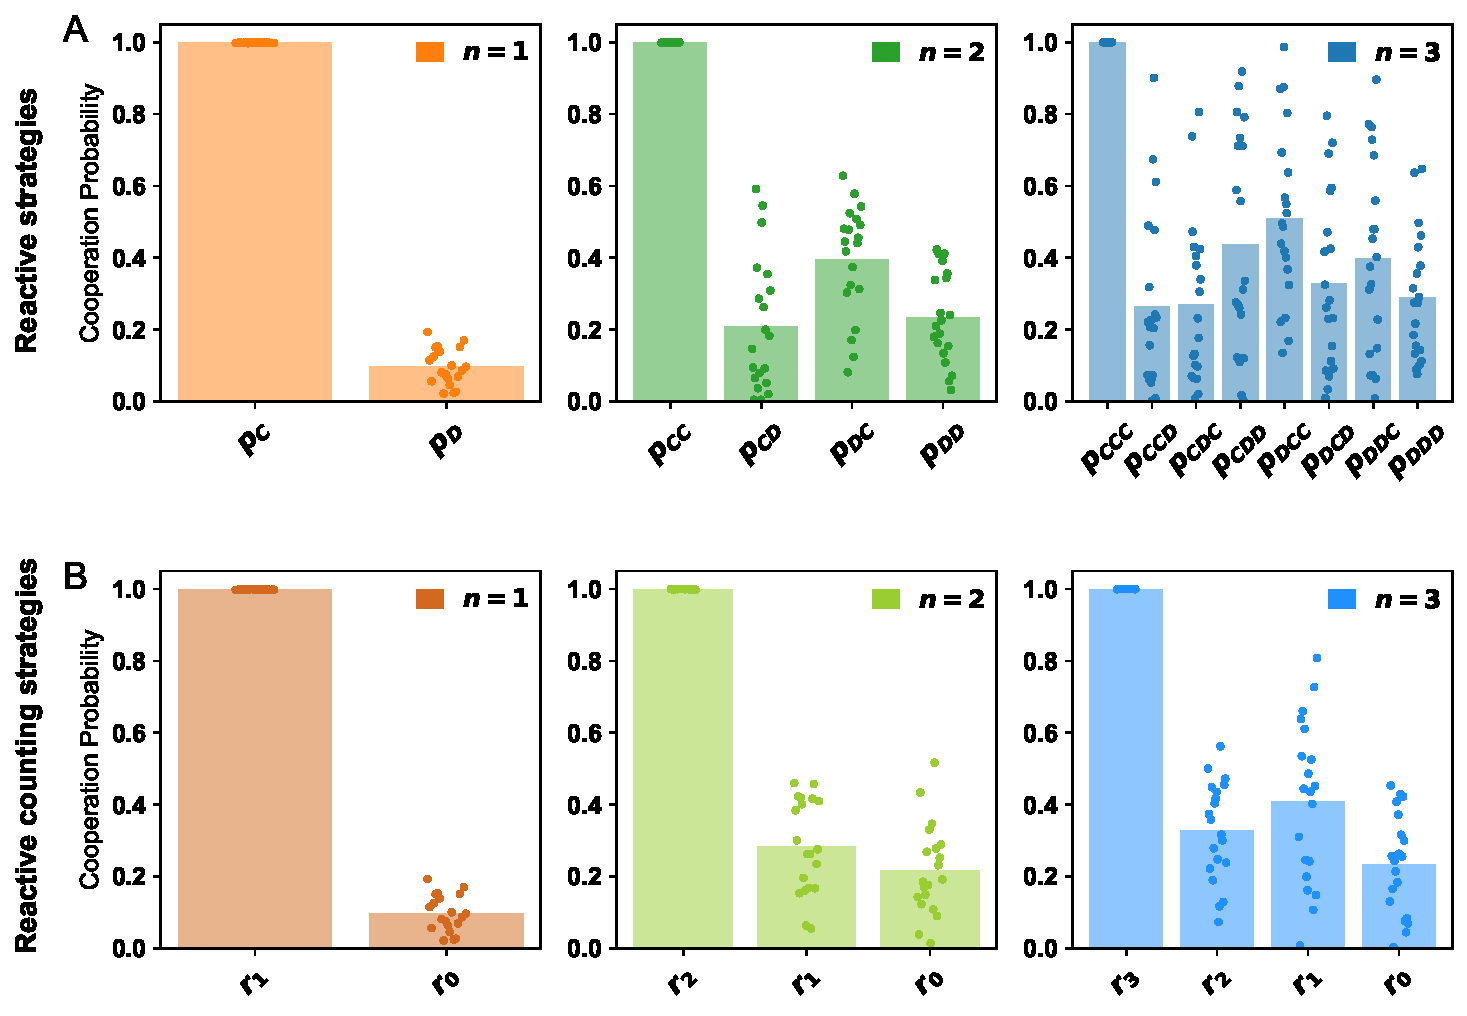
\includegraphics[width=\textwidth]{../../figures/siFig3AbundantStrategies.pdf}
    \caption{\textbf{Evolutionary dynamics of reactive-$n$ strategies.}
    To explore the evolutionary dynamics among reactive-$n$ strategies, we run simulations based on the
    method of Imhof and Nowak. 
    This method assumes rare mutations. 
    Every time a mutant strategy appears, it goes extinct or fixes before the arrival of the next mutant strategy. 
    We run twenty independent simulations for reactive-$n$ strategies.
    For each simulation, we record the most abundant strategy (the strategy that resisted most mutants). 
    The respective average cooperation probabilities are in line with the conditions for partner strategies. 
    Simulations are based on a donation game with \(b\!=\!1\),  \(c\!=\!0.5\), a selection strength $\beta\!=\!1$
    and a population size $N\!=\!100$, unless noted otherwise. For $n$ equal to 1 and 2, simulations are run for \(T\!=\! 10 ^ 7\) time steps. For $n\!=\!3$ we use \(T\!=\! 2 \!\cdot\!10 ^ 7\) time steps.
    }\label{fig:evolutionary_results}
\end{figure}

\subsection{Invasion Analysis}

One question that arises is that from these top strategies which are partner
strategies, and why are some partner strategies selected more than others. For example
in the case of reactive 1, we take a reactive strategies to be ($p_{C} > 0.95$) and
($p_{D} < \frac{c}{b}$), hwer we osbset strategies of ($p_{D} = 0.1$) and closer
to the boundy. The reason for this is exaimpled by Figure~\ref{fig:InvasionAnalysisReactiv1}.


\begin{figure}[tbhp]
  \centering
  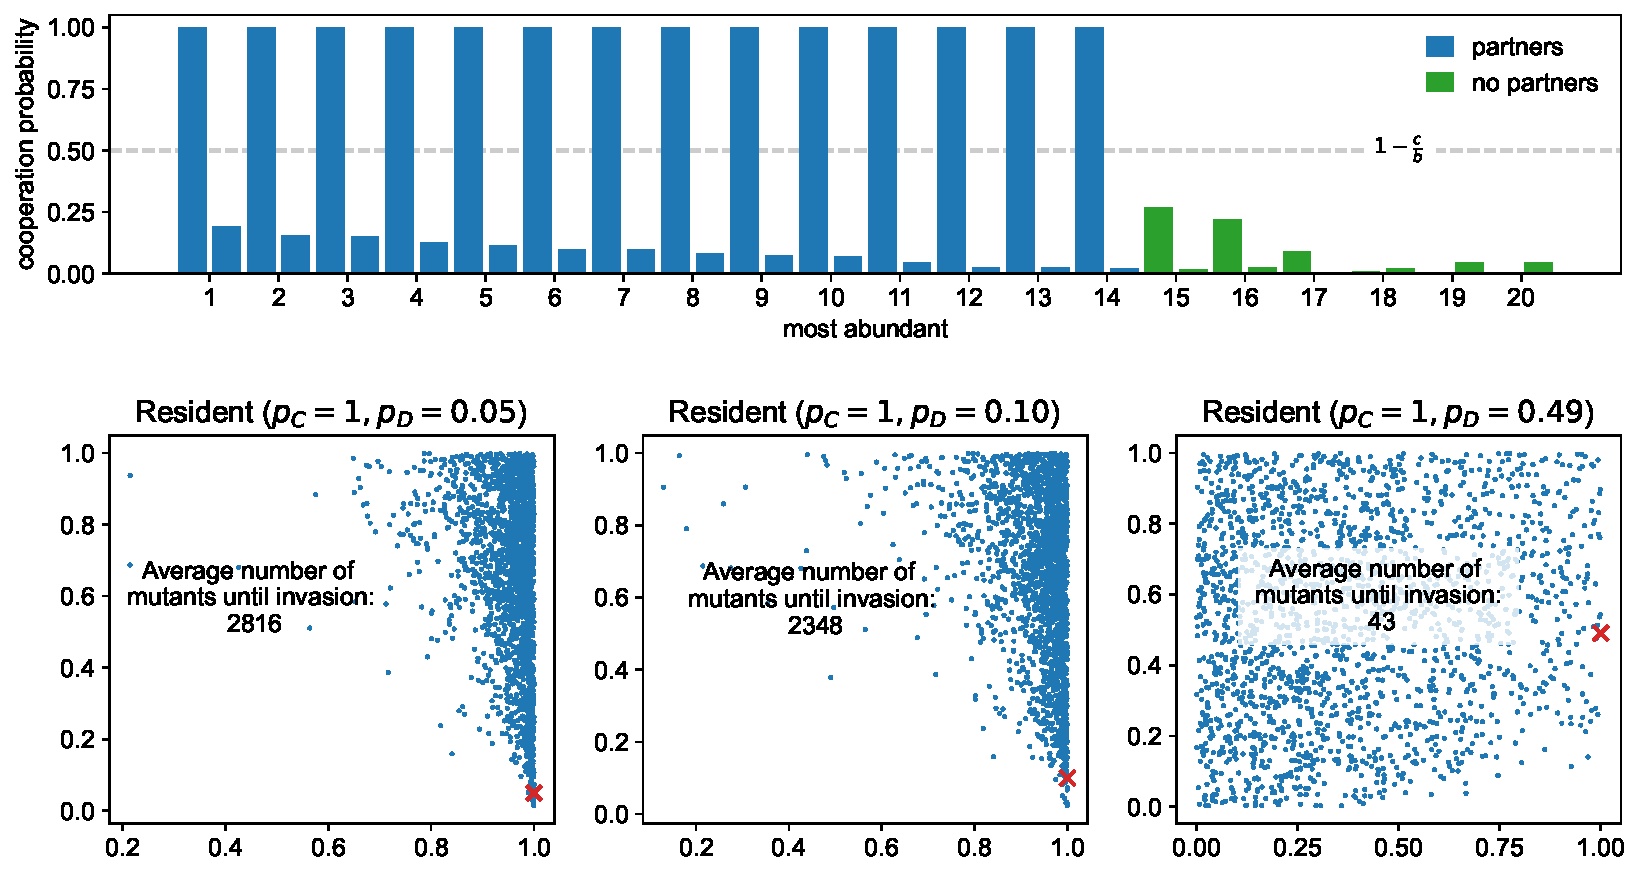
\includegraphics[width=\textwidth]{../../figures/siFigInvasionR1.pdf}
  \caption{\textbf{Invasion analysis for reactive-1.}
  \textbf{A} The twenty most abundant reactive-1 strategies of Figure. We obsvere
  that all twenty of them are partner strategies, and than all have a very low p > 0.2.
  \textbf{B} We perform an invision analysis. Namely we select one resident and we
  introduce mutatns until the mutant takes over and the resident is no more. We count
  how many time from 10 ** 3 a mutatn succeffully invaded the resident. We repeated this
  for three different resisndetd, from left to right. We Obseverd that a resident
  with a very lowp_d is more resistant to invasion, and thus why we observe that
  the most abundant strategieshave a low pd.
  \textbf{C} We can exaiple the low pd if we consider the expected payoff of the three
  resindets when \(k\) ALLD mutatns try to invavde. We can see that for the far left resident
  the expectedpayoff is almost always strivly higher than that of the ALLD mutatns, only whe
  99 mutatn the payoff is the same. We repeated this for all three.
  \text
  }\label{fig:InvasionAnalysisReactive1}
\end{figure}

\begin{figure}[tbhp]
  \centering
  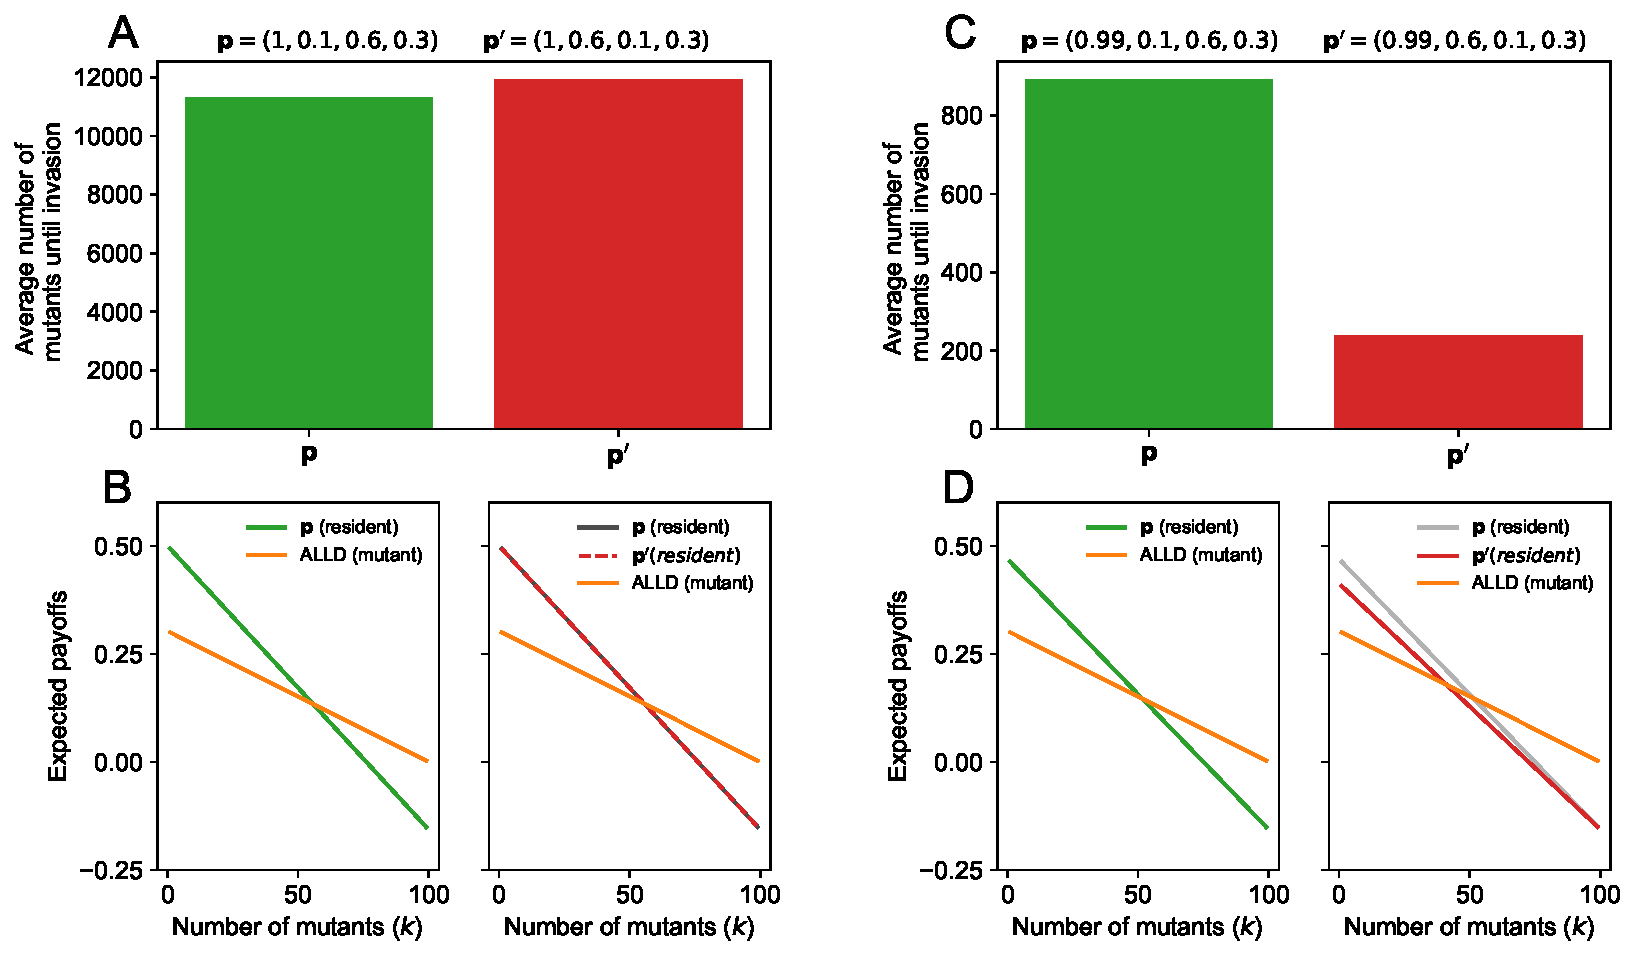
\includegraphics[width=\textwidth]{../../figures/siFigInvasionR2.pdf}
  \caption{\textbf{Invasion analysis for reactive-2.} We repeate the same
  analysis for the reactive-2 strategies. The twenty top performing strategies
  are again partner strategies. Howver, what we observe here is that the
  partner strategies that are selected from the evolutionary process
  almost laways have a smaller pcd than pdc and a low pdd. We already discussed
  why a smaller pdd is selected. Howver, to understand the differencesbetween
  we will consider two examples of such strategies. Namely let $\mathbf{p}=$
  and $\mathbf{\tilde{p}}$. We run an invasion analysis to see the difference
  and inddeed p is invaded much faster. The expected payoffs show that the
  slef payoffs od the strategies are different, and thus an alld recived
  a higher payoff with less mutants.
  }
\end{figure}

The self payoffs of the two strategies would have been the same if p was
equal to 1. However, since the evolutionary process almost never samlples such
a strategy a stochastic pcc makes the difference. The likelyhood of both strategies
to make a mistake while at the outome is the same. Howver, the distributions of
the playing with themselves is different. The numerical evalution of the stateionary
distribution is shown in Figure A. We also use the open source package Axelrod
to simulate the play betwwen the strategies. We run each match for $10^6$ steps
and we repeate the match twenty times. From Figure B we see that the simulation
estimtes the stattionary distribution with the numerical approach. 

From the simulation we can record how long it takes for each pair to return
to mutual cooperation after a mistake has occure. This is shown in Figure C.
We can see that the pair p has a smaller cycle which means it can correct the
mistake faster.

We can look into some of the cyles. The most common cycles for each are those
of the nature, cc|cc and then. SHow in Figure 3, A and B. 

Now we ask the question, what if the lower probably of this path was to be a defection
instead of a cooperation. What we see is that for p rime it takes one extra
timestep tp correct the mistake. This comes from the effect that to go to mutual
cooperation a defection in the second to last round will be at the memory of the
strategy, and a more forgiving strategy achieves mutual cooperation again faster. 



% \noindent
% \textbf{Reactive-1 strategies.} In the case of reactive-1, all the most abundant
% strategies are partner strategies. However, from Eq. and for a given value of c,
% the probability of defecting is... However, we observe only a lower value of \(
% p_{dd} \), thus only some partner strategies are residents. This result is not
% explained by the theory. To better understand this result, we need to do an
% invasion analysis. For the invasion analysis, we consider a given resident
% strategy, and we sample \( 10^3 \) random strategies to estimate if this mutant
% will invade the resident. We record the number of mutants that took over. We
% repeat this \( 10^3 \) times. The results are shown in Fig. X, and what we
% observe is that a lower value of \( p_{dd} \) results in a more robust strategy
% to invasion, as only cooperative strategies on the GTFT can take over, in
% comparison with panel B where defective strategies are more likely to invade.

% \noindent
% \textbf{Reactive-12strategies.} In the case of reactive-2, we observe that almost all
% strategies are partner strategies. However, what seems to be the case is that \(
% p_{dc} \) is higher on average than \( p_{cd} \). In order to understand this,
% we again run an invasion analysis. This time we also consider two values of \(
% p_{dd} \). The results are shown in Fig. Y. \\


%%%%%%%%%%%%
%% Errors  %%
%%%%%%%%%%%%

\newpage

\section{Errors}

So far, we have considered the case where there cannot be a mistake in the
actions taken by a player; the actions of the players are realized without
error. Here, we discuss what happens in the case where such an error is
possible. More specifically, we consider that \(\epsilon\) is the probability
that a player makes a mistake in the action taken.

\begin{figure}[t]
    \centering
    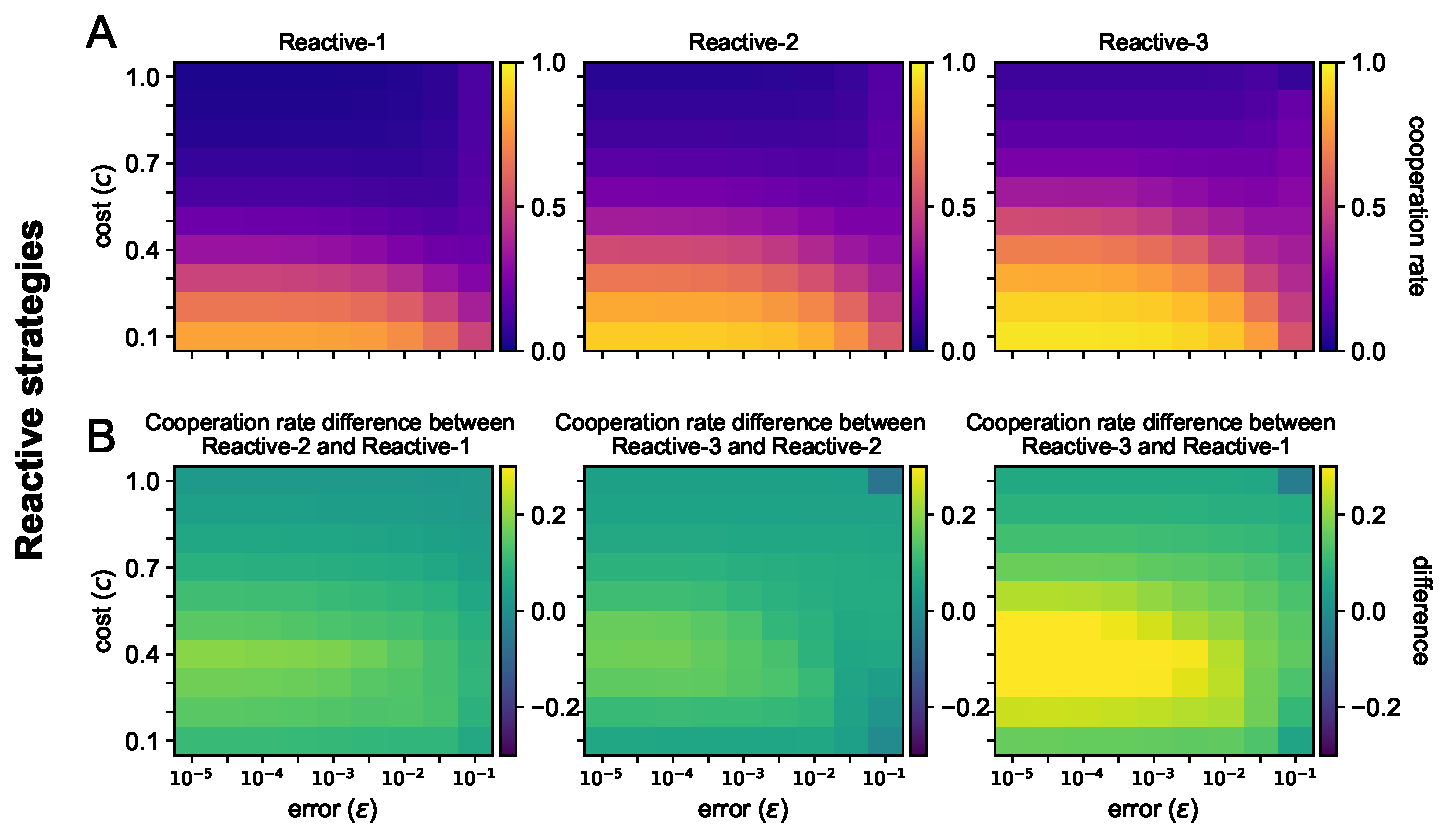
\includegraphics[width=\textwidth]{../../figures/siFig2Errors.pdf}
    \caption{
    \textbf{Cooperating rates with implementation errors.}
We simulate the evolutionary process, this time allowing for implementation
errors. Specifically, we consider a probability \(\epsilon\) that a player makes a mistake
in the action taken. We calculate the average cooperation rate for different
values of \(\epsilon\) and \(c\).
{\bf A} We plot the average cooperation rate for the different parameters when
individuals use reactive-1, reactive-2, and reactive-3 strategies, respectively.
{\bf B} We plot the differences between the cooperation rates when individuals use
different memory size strategies. From left to right, we show the differences
between reactive-1 and reactive-2, reactive-2 and reactive-3, and reactive-1 and
reactive-3 strategies.
    }\label{fig:errors}
\end{figure}

\begin{figure}[h]
  \centering
  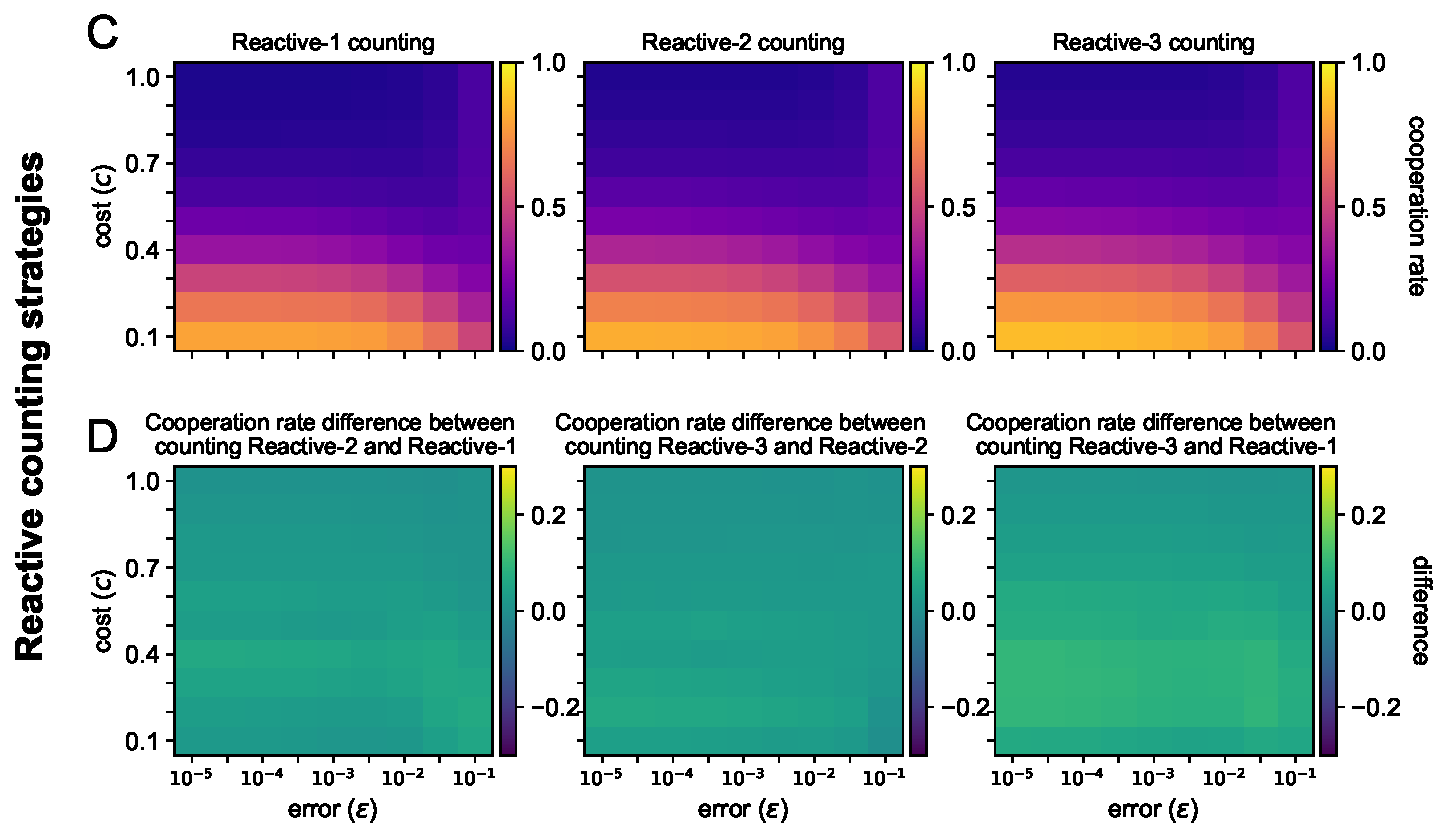
\includegraphics[width=\textwidth]{../../figures/siFigErrorsCounting.pdf}
  \caption{
  \textbf{Cooperating rates with implementation errors.}}
\end{figure}


\newpage

\section{Memory-$n$}

So far in the evolutionary simulations we have considered reactive strategies,
and we have shown that strategies with larger memory allow for more cooperative
populations. We repeate the evolutionary simulations but this time using memory
n strategies. We get results for memory-1, memory-2 and for memory counting
strategies for n equal to 1, 2 and 3. We omit memory-3 strategies because it
is numerically untractable to run such simulations. The results still hold.
For more memory more cooperation evovles, howber, not in the case of counting
strategies.

\begin{figure}[t]
  \centering
  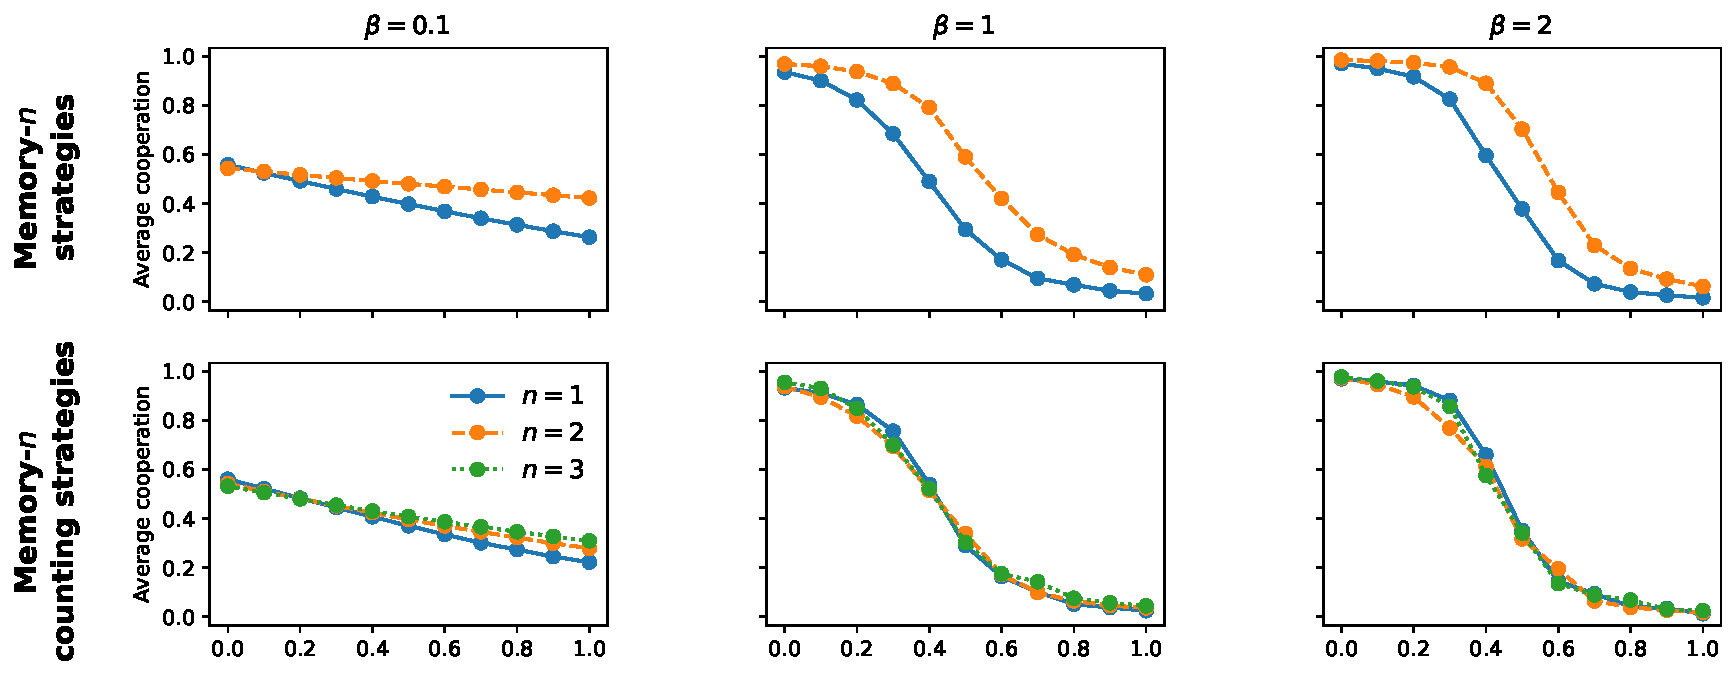
\includegraphics[width=\textwidth]{../../figures/siFigMemorySim.pdf}
  \caption{
  \textbf{Memory-$n$ simulations.}}
\end{figure}


To understand why counting strategies do not allow for more cooperation we focus
on reactive-2 strategies and reactive-2 counting strategies. We run an invasion
analysis where we select the most abundant reactive-2 strategy and hte most
abundant reacto-2 coutning strategy. The strategies and the mean invasion
time are given by Figure 3. We also ask the question, how many reactive-2
mutants can a reactive-2 coutnign strategy repel.

\section{Proofs}

The proof for Theorem 1.

The proof for Theorem 2.

\end{document}